% Section content template for individual Educative lessons
% This file contains the actual content for a specific section
% Generated from Educative API section content

% Section: Sequence Diagram for the Hotel Management System
% Section ID: 4909350250610688
% Section Slug: sequence-diagram-for-the-hotel-management-system
% Generated: 2025-12-12T16:23:35.482890

Sequence diagrams are a great way to understand the interactions between different entities and objects in the system. There can be different sequence diagrams that we can create for our hotel management system. In this lesson, we will create sequence diagrams for the following two interactions:

\begin{itemize}
\item
\protect\phantomsection\label{z4YjEL15iBQRdmpCly2on}
\textbf{Book a room:} The guest books a hotel room online.
\item
\protect\phantomsection\label{fG1hXUIHSvxemUddQMdzs}
\textbf{Sequence challenge:} The guest checks out of their room at the reception.
\end{itemize}

\subsection{Book a room}\label{bPjnJLd68-tBGqb1P3u_U}
\\
The sequence diagram for the room booking should have the following actors and objects that will interact with each other:

\begin{itemize}
\item
\protect\phantomsection\label{L3hJa50USjnMXiih_qPHC}
\textbf{Actor:} \texttt{Guest}
\item
\protect\phantomsection\label{81ksXql5w5Lcr9a10EOFB}
\textbf{Objects:} \texttt{Catalog}, \texttt{Booking}, \texttt{Room}, and \texttt{Payment}
\item
\protect\phantomsection\label{Z-FJ7LOHFTa5GtBeukGLq}
System
\end{itemize}
\\
Here are the steps in the book room interaction:

\begin{enumerate}
\item
\protect\phantomsection\label{_birp3wlA1zLx5mtHHKYA}
The guest searches for a room based on price and style.
\item
\protect\phantomsection\label{pr79H-MAXxFd7xbPNf7dh}
The catalog returns a list of rooms.
\item
\protect\phantomsection\label{3yq8XOkIaVq2OBKUn5D1k}
The guest selects a room they wish to book.
\item
\protect\phantomsection\label{aESY_0fGiSzHgidnCYOhL}
If the room is available:

\begin{enumerate}
\item
The guest creates a booking for the room.
\item
The booking fetches the booking price for the room.
\item
The guest is informed that the booking is ready for payment.
\item
The guest initiates a payment against the booking price.
\item
The payment is processed, and the guest is informed of the status.
\item
If the payment is successful:

\begin{enumerate}
\item
The guest is informed that the payment has succeeded.
\item
The system is informed that payment is complete.
\item
The system updates the room status to reserved.
\end{enumerate}
\item
Else if the payment is unsuccessful:

\begin{enumerate}
\item
The guest is informed that the payment has failed.
\end{enumerate}
\end{enumerate}
\item
\protect\phantomsection\label{BE9GVOC0wL34n_11AaRsR}
Else if the room is unavailable:

\begin{enumerate}
\item
The system informs the guest that the room is unavailable.
\end{enumerate}
\end{enumerate}
\\
Based on the order above, the sequence diagram of booking a room in a hotel management system is given below:

\begin{figure}[htbp]
 \centering
 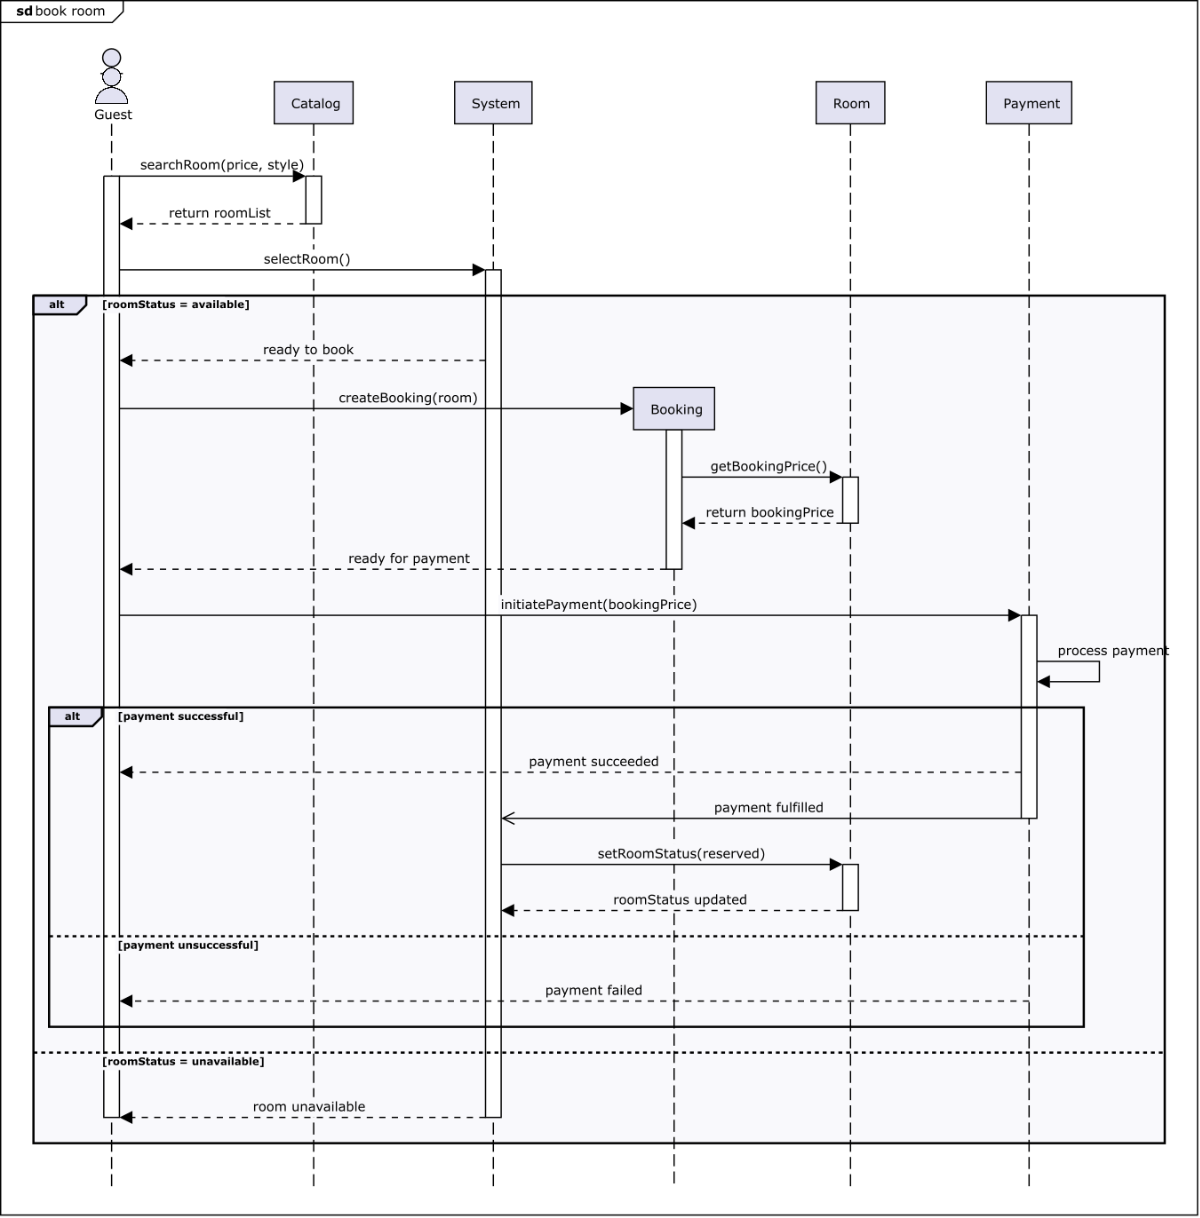
\includegraphics[width=0.5\textwidth]{Images/chapter_18/section_4909350250610688/4991626038738944.png}
 \caption{The sequence diagram for online room booking}
\end{figure}

\subsection{Sequence challenge: The housekeeper performs maintenance in a room}\label{fHxT_dVYp6FmPOr1CFhnN-1}
\\
You will help us complete a sequence diagram for the housekeeper who performs maintenance in a room.
\\
A skeleton of the sequence diagram is provided below.

\begin{figure}[htbp]
 \centering
 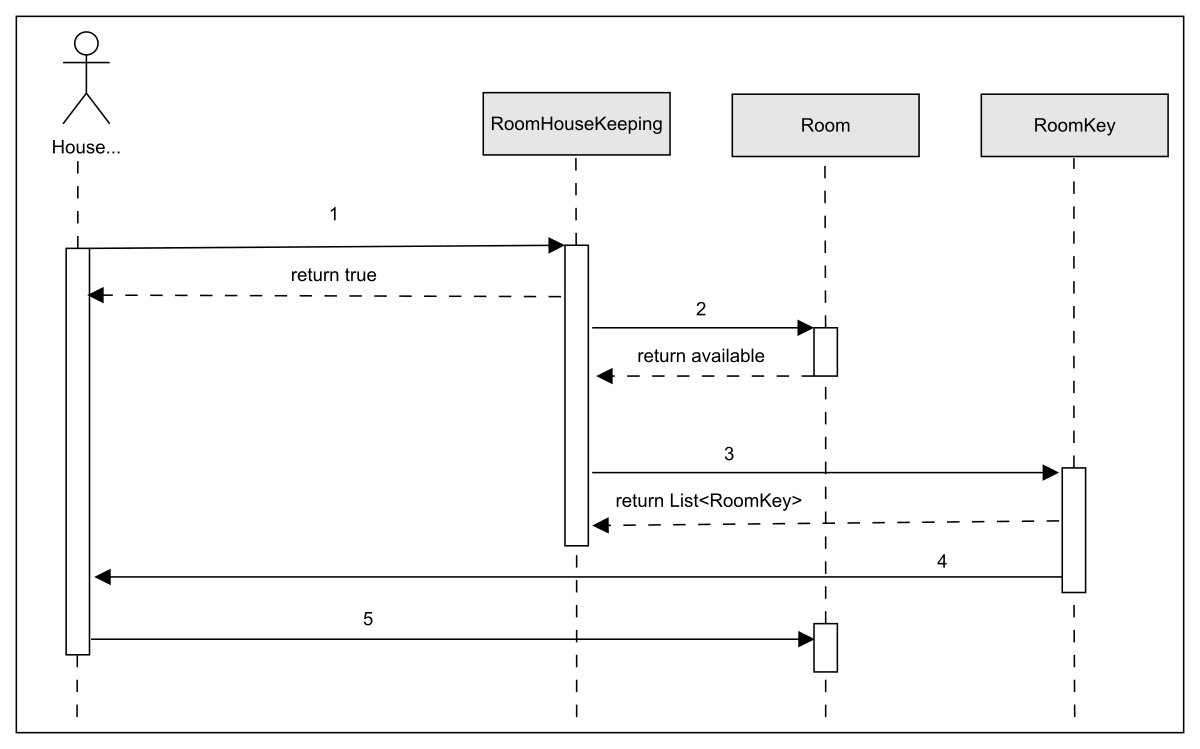
\includegraphics[width=0.5\textwidth]{Images/chapter_18/section_4909350250610688/6166886973571072.png}
 \caption{The sequence diagram for checking out of the hotel}
\end{figure}

Notice that the arrows in the diagram above are numbered from 1 to 5. Below are the messages between the actor(s) and object(s). Can you rearrange the messages below in the correct order sequence they should appear in the skeleton of the sequence diagram above?
\begin{quote}
\textbf{Note:} If you're stuck, click the ``Show Solution'' button.
\end{quote}

In the next lesson, we'll create activity diagrams for the hotel management system.

% End of section content